% !TEX root = defense_index.tex

% Wow that was a silly thing to put up front
%\begin{center}
%``Qui custodiet ipsos custodes?''
%\par
%Juvenal's Satire VI
%\end{center}

% Use a theme of communication: it is central to electrical engineering and encapsulates the activity of the brain
% It also serves well to discussing how clinicians `communicate' their results and for the techniques applied to process EEGs

The ability to communicate underlies the major functions of the brain. Given the array of tools at our disposal (voice, facial expressions, hands, feet and eyes) our ability to communicate is limited only by our inventiveness. However, this system of communication limits our brain by forcing it to indirectly communicate through these tools. When we wish to study the brain itself problems arise because the majority of measurements come through indirect means. This is further complicated as the ideas to be expressed become more complex either in terms of emotional context or severity, such as pain and illness.

Presently, electroencephalography is the principle method of directly communicating with the brain. While the communication is one directional, in that we can only listen, it affords opportunities not available through our human faculties. \acp{EEG} may be used to discern the incidence of epilepsy and stroke \cite{Markand2003}, study neural responses to stimuli \cite{Picton1992}, or even neural control feedback \cite{Khanna2016}. Recently, the advent of inexpensive commodity-grade \ac{EEG} headsets \cite{Liao2012} has expanded the field to include areas such as gaming, neuro-modulation, and mindfulness training \cite{Lance2012}.

These advances allow for direct and more timely interpretation of \acp{EEG} via the creation of digital signal processing tools that can identify or predict neural activity \cite{Ramgopal2014}. In clinical settings this technology assists neurologists in reviewing long recordings \cite{Lopez2015}, communicating with patients \cite{Picton1992}, and processing artifacts \cite{Nolan2010}. These tools leverage multidimensional statistical models \cite{Schulz2012, Kannathal2005, Lawhern2016} to enhance our understanding of \acp{EEG}. In research settings, this technology has facilitated advances in \acp{BCI} \cite{Lotte2010b} and seizure prediction \cite{Chu2017}.

Historically, computer-based \ac{EEG} interpretation has been only moderately effective despite large quantities of research \cite{Wulsin2011,Vidaurre2011b}. One key problem is that brain function (and by extension an \ac{EEG} recording) is highly variable, requiring very large sample sizes in order to create robust statistical models \cite{Stober2015}. The most powerful statistical methods generally require even larger samples sizes to assure convergence \cite{Izenman2008}. Until recently it has been difficult to collect, store, and process such large \ac{EEG} datasets.

Modern digital data collection methods, in both clinical and research settings, have made `big neural data' feasible \cite{Obeid2016a}. However, these datasets must be \emph{annotated} prior to being useful for training statistical models. Annotated data is produced when an expert reviews the recordings by marking which segments of the recordings correspond to known phenomena \cite{Kaplan2013}. These annotations can be at the macro scale (such as `seizure') or the micro scale (such as `sharp spike wave'). Not surprisingly, \ac{EEG} annotation is manually intensive making it rarely cost effective to ask clinicians to perform it at a fine-grained level \cite{Tsiouris2015}

% Figure here to illustrate what/why/how annotations come about

There are communication problems between even well trained clinicians on how and what to annotate on recordings. This is evident by moderate consensus agreement when annotating simple events such as variations of spike waveforms \cite{Grant2014,Gaspard2014,Halford2015,Warby2014}. Conflicting annotations make it difficult to produce `gold standards' of annotations used for training new clinicians and for leveraging the power of \emph{supervised} \ac{ML} techniques.

Supervised \ac{ML} techniques rely on this annotated data, more commonly called \emph{labeled} data within the \ac{ML} community, to produce sufficient models of known classifications. By using prior knowledge of the data, models can be trained to classify previously unseen data in classes such as background, seizure, and sleep. However, a common problem with these techniques is a lack of strong consensus for each class \cite{Ramgopal2014}. Thus the system is inherently limited by the quality and quantity of its prior knowledge.

The difficulty increases when building \emph{unsupervised} \ac{ML} techniques that operate on unlabeled data \cite{Tsiouris2015,Ghosh-Dastidar2007}. Now the techniques are tasked with first determining how to partition the data into classes and then performing classification on those self-generated labels. This typically requires additional data beyond a supervised approach, but removes the stipulation of prior knowledge.

Despite the majority of research focusing on supervised \ac{ML}, an unsupervised \ac{ML} method may best suited for interpretation of \acp{EEG}. Unsupervised approaches are decoupled from clinicians because there is no need for labeled data. Clinicians are capable annotators, but even in their area of expertise they have biases which manifest in poor inter-rater agreement when aggregating annotations \cite{Halford2017}.  Furthermore, as the use cases of \acp{EEG} grow they advance beyond what clinicians typically annotate, meaning it is impossible to provide a documented ground truth. Given such constraints, this work introduces \acp{IV} as an unsupervised machine learning method for \acp{EEG} with the aim of supplanting the reliance on clinician annotations.

%%%%%%%%%%%%%%%%%%%%%%%
\section{The Landscape of Electroencephalograms}

Before outlining the aims of this work, a brief background is provided to a shared understanding of the relationships between \acp{EEG}, algorithms and clinicians. Chiefly among these relationships is the way in which algorithms and clinicians are trained and perform annotations. Specific attention is paid to how clinicians, as individuals and groups, produce the annotations used for algorithm development. The performance of these algorithms is outlined to contrast with the scope and performance of their human counterparts. Attention is focused on the algorithms areas of application and performance.

%%%%%%%%%%%%%%%%
\subsection{Clinician Development}

Clinicians undergo extensive training, often culminating in a fellowship to specialize in the treatment of epilepsy, sleep disorders, or intensive care. These specializations require the ability to interpret \ac{EEG} recordings\footnote{Taken from: \url{https://medicine.yale.edu/neurology/education/fellowships/epilepsy_eeg/}} for which the clinician can be certified through the \ac{ABPN}. The \ac{AAC} works with the \ac{ABPN} to ensure clinicians are adequately trained, but cautions that ``[N]ot all hospital credentialing boards require sub-specialty training to allow individuals to interpret \acp{EEG}''\footnote{Taken from: \url{https://www.aan.com/uploadedFiles/Website_Library_Assets/Documents/4.CME_and_Training/2.Training/3.Fellowship_Resources/3.How_to_Apply_for_a_Fellowship/Epilepsy\%20Fellowship\%20FAQ.pdf}}. Sub-specialty certifications are limited to topics such as brain injury, neuromuscular issues, and epilepsy.

Beyond this, clinicians refine their skill on the patients they encounter through their practice of medicine. Principle among these skills is their ability to accurately annotate \acp{EEG} recordings. Annotations focus on documenting the activity of the brain via signals recorded from strategically placed electrodes extracranially (on the scalp) or intracranially (on the surface of the brain) \cite{Epstein2006}. The methodology of annotating and interpreting \ac{EEG} recordings is part of the certification process, but the Epilepsy Foundation contends that ``EEG training for clinicians is inadequate''\footnote{Taken from: \url{http://www.epilepsy.com/article/2014/12/eeg-training-clinicians-inadequate}}. In spite of this, clinical annotations remain the best tool for assessing the behavior and state of a brain \cite{Banaschewski2007}. 

Even with all their training and successful treatment of the myriad of brain disorders, clinicians are not without their inconsistencies as they are human \cite{Grant2014}. Firstly, their ability to annotate accurately is often surpassed by the amount of data produced from tests. This leads to annotation consuming a disproportionate amount of their work hours. Secondly, their formal education ensures they are in agreement on terminology and its manifestation \cite{Gaspard2014}. However, performance in consensus-bases studies suggests there are disagreements over which waveforms are of interest to each clinician \cite{Grant2014,Halford2015,Warby2014}.

Thus it is clear that clinicians are capable interpreters because they readily determine the correct diagnosis from a \ac{EEG} recording. However, their reasoning for these assessments have the potential to be disparate. This behavior is not unique to a specific subset of conditions as it is readily apparent in the lack of annotation consensus in sleep \cite{Warby2014}, seizure \cite{Grant2014} and cardiac \cite{Westhall2015} \ac{EEG} recordings.

Even when presented with data common to their expertise, pairwise clinician similarity (Cohen's $\kappa$ statistic\footnote{The statistic is not perfect \cite{Gwet2002}, but does appear to be among the most common reported in studies assessing neurologist performance.}) is moderate (0.41-0.60) at best \cite{Grant2014} and group performance varies from slight (0.0-0.20) to almost perfect (0.81-1.00) \cite{Westhall2015}. This suggests clinicians identify different, but valid, indicators of disorders. Ultimately this produces multiple divergent, but correct, sets of annotation from one dataset. While not problematic for diagnosing disorders, it makes it difficult to develop \ac{ML} algorithms when there are multiple `right' answers.

%%%%%%%%%%%%%%%
\subsection{Clinical Annotations}

The ability to produce correct annotations is a fundamental component of \ac{EEG} based research. In order to validate the performance of algorithms, clinicians must provided annotated data. These datasets are annotated through the lenses of the clinician's specialization and the patient's condition or diagnosis. As discussed previously, even when annotating the same data, clinicians struggle to come to consensus about its contents. Figure \ref{fig:halford_anno} shows the results of seven clinicians annotating an hour long segment for seizures and \acp{PD}. Nearly all the clinicians annotate abnormal events, save one, but the diversity and quantity of annotations are inconsistent.

%%%%%%%
\begin{figure}
\centering
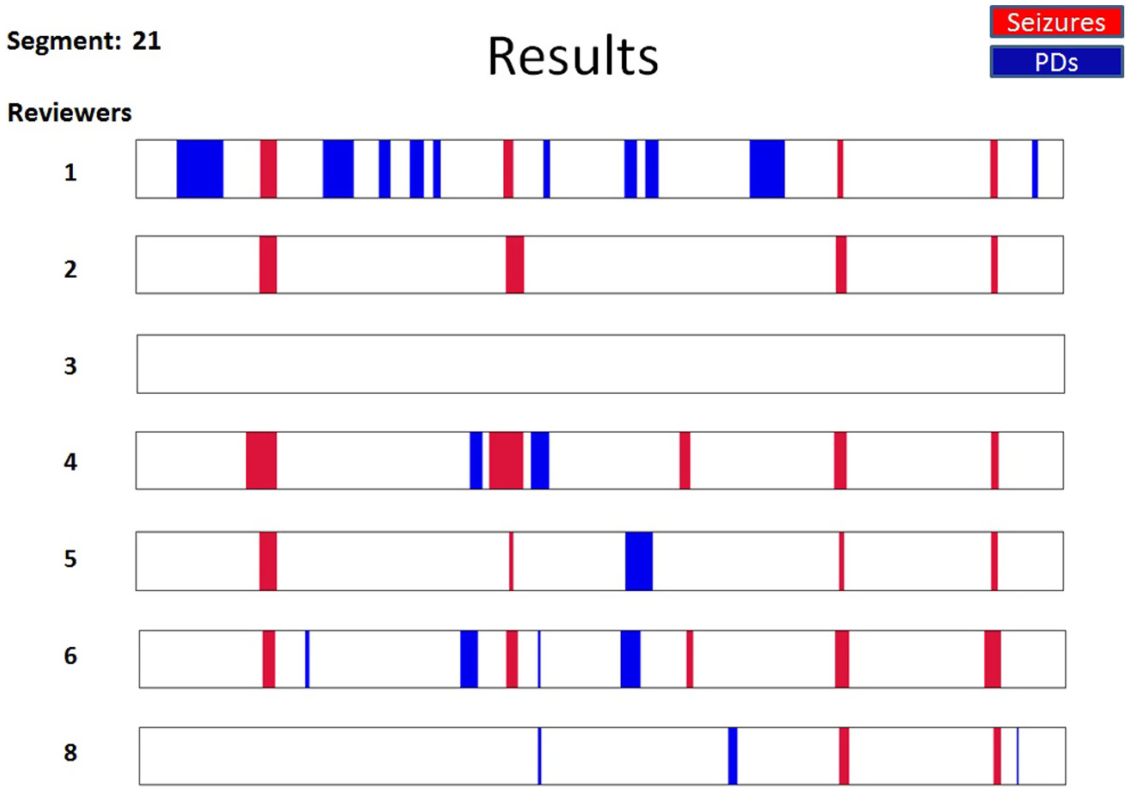
\includegraphics[width=0.6\linewidth,keepaspectratio]{halford_7rev}
\caption[Example of EEG]{In Halford et al. \cite{Halford2015}, seven reviewers were asked to annotate for seizures and \acp{PD}. The annotation results of the hour long recording, Segment 21, show that six reviewers labeled seizure events, five labeled \acp{PD}, and one labeled nothing. The quantity of annotation varies as does the spatial alignment between between reviewers.}
\label{fig:halford_anno}
\end{figure}
%%%%%%

Further complicating matters is that investigators often produce their own datasets, specifically for a given study. This occurs because existing datasets lack annotations, subject information, recording parameters, or protocols necessary to address their specific research questions. This makes it difficult to reuse previously annotated data because there is nothing is standardized. While one study annotates the other two do not, and then all three present with different sampling rates, recording durations, and electrode layouts.

% May need to cite something here, or perhaps an image from a study
While these decisions are practical with respect to specific studies, this behavior prevents supervised \ac{ML} techniques for being applied across datasets. Without consistent sampling rates, the datasets may need to be interpolated to produce consistent windows of data. Mismatches in electrodes, inconsistent annotations, and artifacts are often manually resolved via the experiment team's limited knowledge or by possibly requiring the assistance of yet another clinician. While algorithms may overcome noise inherent in the data, this is only possible if there is a plethora of well annotated data from which to learn.

Annotations start, as shown in Figure \ref{fig:wulsin_anno}, as waveforms whose variations conform to similar behaviors. Not all annotations are related to medical conditions, as eye blinks and background are often considered to be noise. Differentiating such noise from waveforms of interest, like \acp{GPED}, \acp{PLED}, spike and sharp wave complexes, and triphasic waves, is a critical step in reading an \ac{EEG}. The \ac{ACNS} defines an exhaustive list of \ac{EEG} terms, including background characteristics, which are outlined in \cite{Westhall2015}. Clinicians are well versed in the terminology, but struggle in their ability to accurately match waveforms with appropriate labels \cite{Gerber2008}.

%%%%%%%
\begin{figure}
\centering
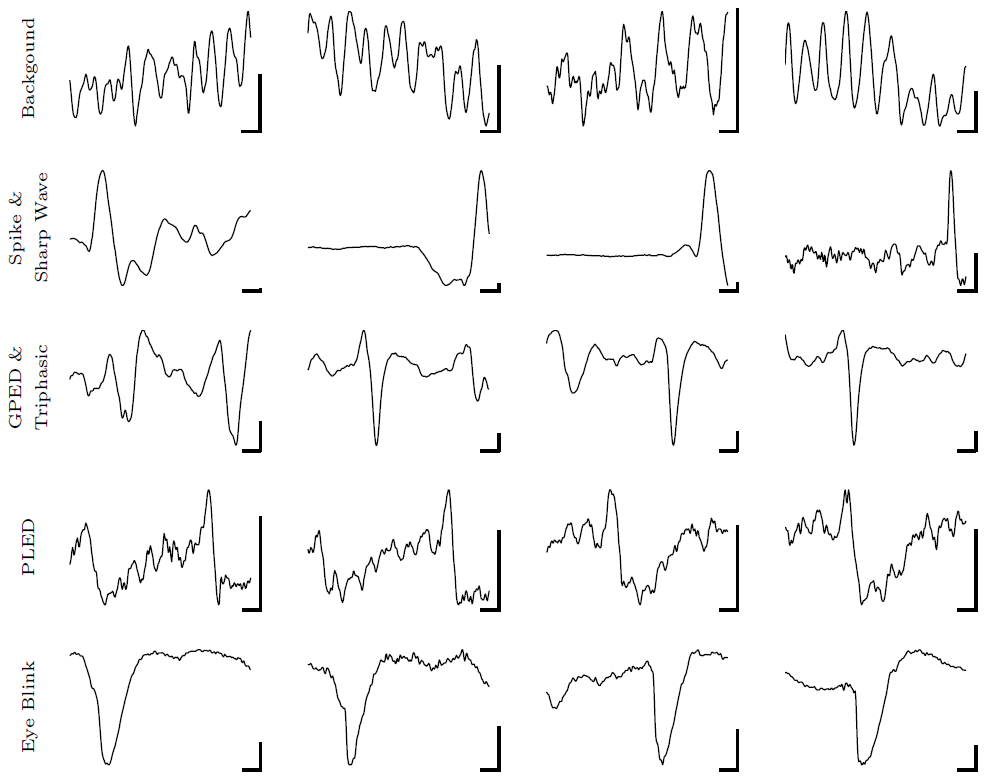
\includegraphics[width=0.6\linewidth,keepaspectratio]{wulsin_anno}
\caption[Annotation example]{Annotations used for the work of Wulsin et al in \cite{Wulsin2011}. Notice the placement of the spike does not need to precede or succeed the sharp wave. \ac{GPED} and \ac{PLED} typically occur over a range of channels making them context dependent.}
\label{fig:wulsin_anno}
\end{figure}
%%%%%%

The waveform examples from Wulsin et al. \cite{Wulsin2011} are drawn from a seizure dataset. However, the waveforms are not unique to seizure recordings and could also be found in any of the other active \ac{EEG} research fields such as attention/workload measurement \cite{Wang2012}, biometric identification \cite{Rocca2012}, \acp{BCI} \cite{Lance2012}, \acp{ERP} \cite{Makeig2012}, and sleep stage classification \cite{Schluter2012}. Each field focuses on different facets of an \ac{EEG} recording and may have distinct waveforms. Other sources for distinct waveforms include subject related traits, such as their age \cite{Warby2014,Clarke2001} and genetics \cite{Begleiter2006}.

In summary, the fundamental technical challenge of training robust algorithms for automatic \ac{EEG} interpretation is the diversity of annotated data. Seizure data differs from \ac{ERP} data which differs from sleep data, making it difficult, if not impossible, to find clinicians capable of accurately annotating all of it. The lack of large diverse sets of thoroughly annotated data encumbers the advancement of algorithm based annotators/classifiers. This is exemplified by the struggle to develop \ac{ML} algorithms capable of meeting performance levels deemed acceptable by clinicians and the inability to produce consistent universal \ac{ML} classifiers.

%%%%%%%%%%%%%%%%
\subsection{Algorithm Applications}

While major research avenues align with clinical applications (sleep, seizure, and various brain disorders), the use of \ac{ML} provides avenues for novel applications as research progresses such as \ac{BCI}, biometric verification, \acp{ERP}, and brain state workloads. Despite the variety of unique classification tasks, they all face similar fundamental performance hurdles. Chiefly among these are the necessary steps of pre-processing to address artifacts and production of acceptable feature sets. Within a given \ac{EEG} recording it can be necessary to address the background waveforms that comprise the majority of the datasets.

\ac{EEG} artifacts are often hard to classify because they appear as waveforms that resemble, Figure \ref{fig:wulsin_anno}, the more critical spikes and sharp waves of seizures \cite{Halford2017} or the natural brain frequency rhythms \cite{Uriguen2015}, Figure \ref{fig:artifactVrhythm}. While artifacts impact clinicians and algorithms, selection of an optimal feature set is unique to the algorithms. This is because feature sets are often paired with the type of \ac{EEG} data being classified. The result is a wide range of potentially useful features consisting of but not limited to \ac{PSD} features \cite{Gui2015}, spatial and temporal features \cite{Mognon2011}, \ac{CEP} feautres \cite{Harati2015a}, auto-regressive parameters \cite{Marcano2018}, and normalized raw data \cite{Acharya2018}.

%%%%%%%
\begin{figure}
\centering
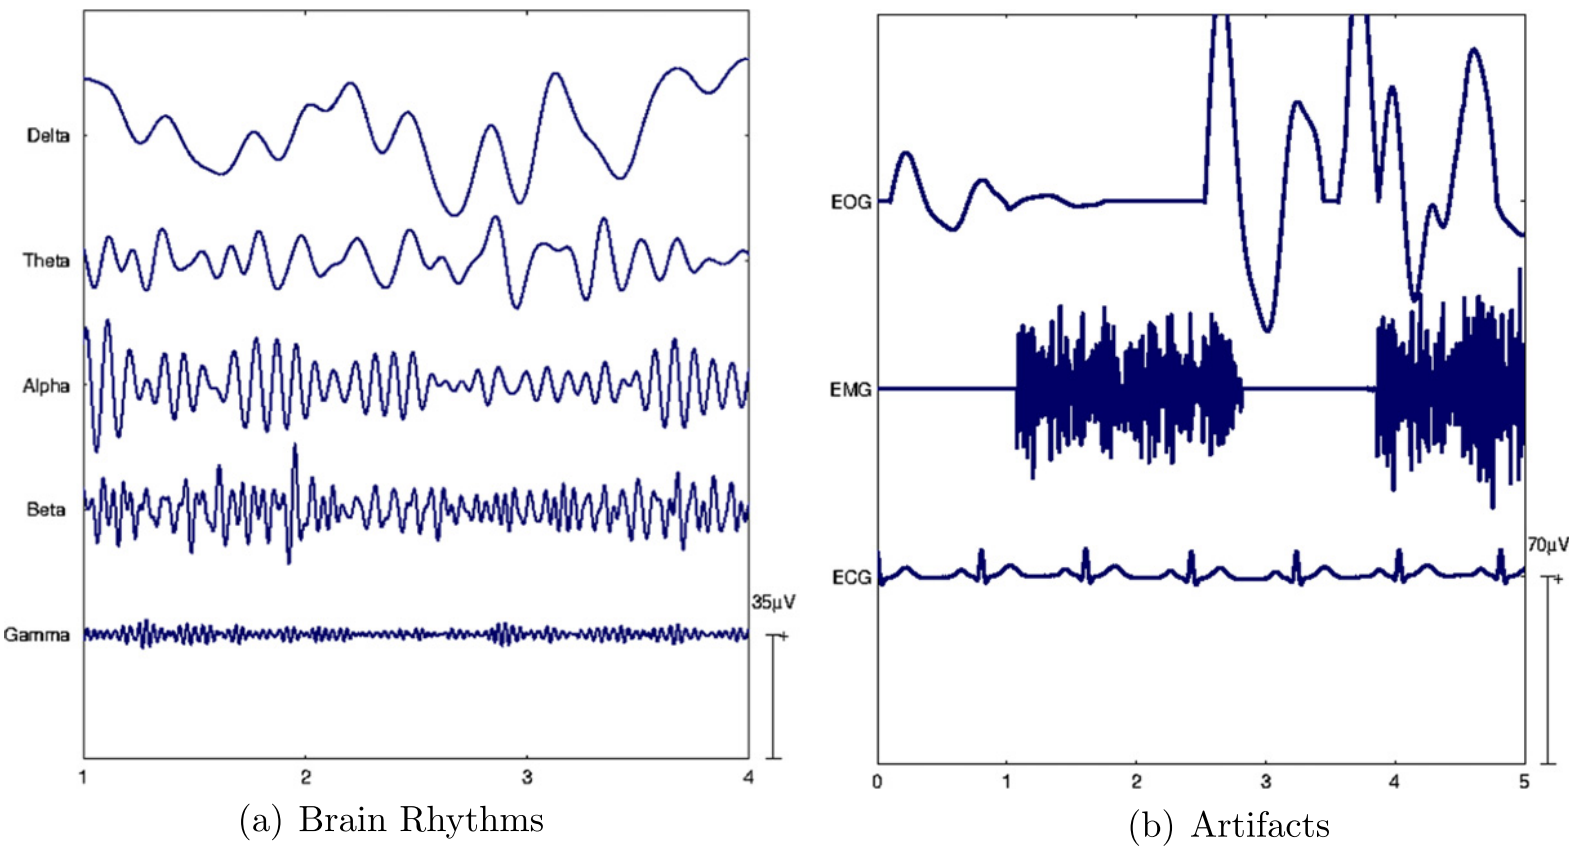
\includegraphics[width=0.8\linewidth,keepaspectratio]{artifactVrhythms}
\caption[Artifact example]{Example of artifacts (b) similarity to the natural rhythms of the human brain (a) used for the work of Uriguen et al in \cite{Uriguen2015}.}
\label{fig:artifactVrhythm}
\end{figure}
%%%%%%

Despite focusing on waveforms of interesting via artifact correction and feature selection, the majority of \ac{EEG} often consists of background signals\cite{Wulsin2011,Rakthanmanon2012,Uriguen2015}. This is frequently a problem for rare events like seizures, but is a boon to subject verification tasks and the biometric community \cite{Campisi2014}. Additionally, there are many less studied conditions that manifest throughout a recording, such as alcoholism \cite{Porjesz2005}, emotional state \cite{Coan2004}, pain \cite{Schulz2012}, and mental focus/workload \cite{Schultze-Kraft2016}.

To motivate the implication of these areas of research a brief review of six common \ac{EEG} classification fields is presented. The use of algorithms for seizure, sleep, \acp{BCI}, \acp{ERP}, and mental/workload classification are readily associated with clinician driven research, while \ac{EEG} based biometrics branch out beyond their well defined knowledge base.

\paragraph*{Seizures}
A substantial portion of work in this field focuses on correctly identifying and locating seizures \cite{Gardner2007,Subasi2007,Wulsin2012,Bogaarts2016}. By isolating seizure events, researchers can focus on the properties of the seizure for the purposes of classification and waveform modeling \cite{Wulsin2011,Blanco2011,Bajaj2012}. The knowledge gained in this process makes it possible to predict seizures in real-time \cite{Ramgopal2014,Chu2017}. Seizure events are typically high energy and frequency wavefroms with synchronization across channels \cite{Halford2015}.

%%%%%%%%%%%%%%%%%%
% figure of brain wave during seizure
\begin{figure}[h]
\centering
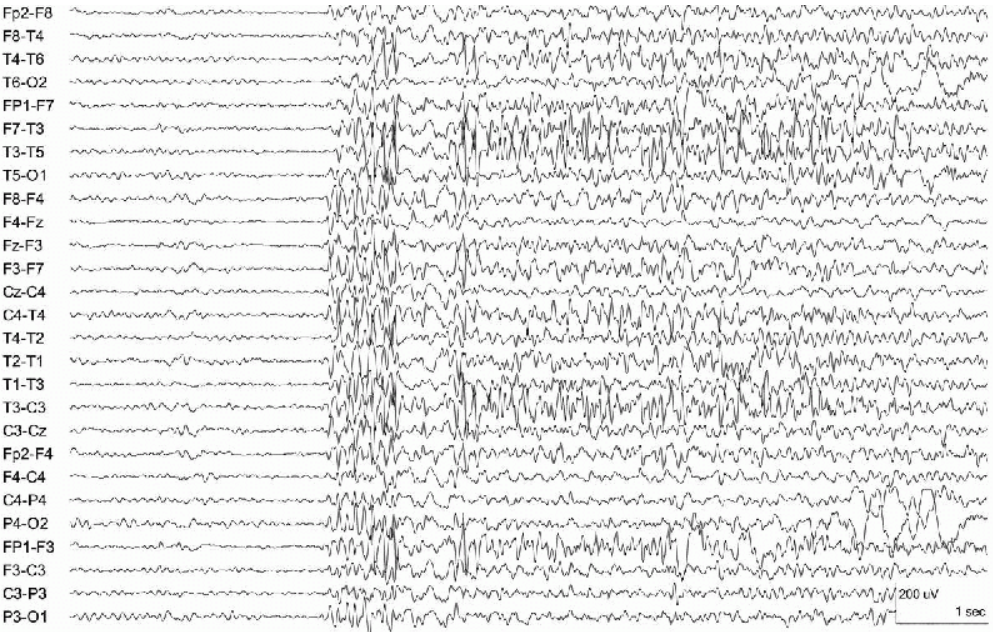
\includegraphics[width=0.75\linewidth,keepaspectratio]{eeg_seizure_generalized}
\caption[Example of a generalized seizure EEG]{A segment of an \ac{EEG} recording taken from a subject at the onset of a generalized seizure. Note that after the seizure starts, activity is not uniform across all channels. Image sourced from Tatum and Tatum\cite{Tatum2014}. }
\label{fig:seizureExample}
\end{figure}
%%%%%%%%%%%%%%%%%%

\paragraph*{Sleep Studies}
Sleep state classification labels the transition from wakefulness to \ac{REM} sleep. Sleeping \ac{EEG} recordings are often cleaner due to lack of movement artifacts which improves their clarity for clinicians and reduces pre-processing for algorithms \cite{Buckelmuller2006}. Despite this and a closed set of distinct stages, sleep stage classification suffers from inter-rater agreement problems \cite{Warby2014}. Sleep spindles and K-Complexes serve as the main indicators of sleep along with pronounced changes in band \acl{PSD} \cite{Wendt2012}. While seizures often manifest during sleep, other issues can also be addressed such as sleep apnea \cite{Schluter2012} and overall brain functionality/health \cite{Zygierewicz1999}.

%%%%%%%%%%%%%%%%%
% figure of brain waves during sleep
\begin{figure}[h]
\centering
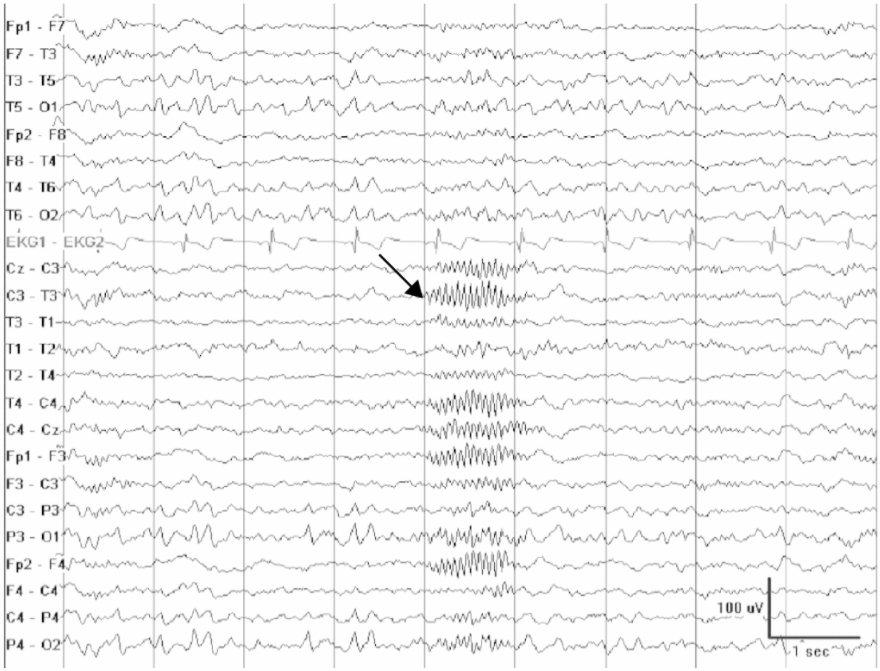
\includegraphics[width=0.75\linewidth,keepaspectratio]{eeg_sleep_N2_sleepSpindles}
\caption[Example of sleeping EEG with sleep spindles.]{A segment of an \ac{EEG} recording taken from a subject in the second of phase sleep. Note the present of sleep spindes, black arrow, across multiple channels. Image sourced from Tatum and Tatum\cite{Tatum2014}.}
\label{fig:sleepExample}
\end{figure}
%%%%%%%%%%%%%%%%%

\paragraph*{Biometrics}
Multiple studies have focused on the use of \acp{EEG} to identify and verify subjects, irrespective of any associated disease and disorder \cite{DelPozo-Banos2014a}. The results of such work suggest that individuals have distinct \ac{EEG} fingerprints \cite{Tangkraingkij2010,Stassen1988,Doppelmayr1998a} which may relate to potential inheritable characteristics \cite{Stassen1988,VanBeijsterveldt2002}. A major theme in biometrics is understanding how different brain states impact these fingerprints. The work of Rocca et al. showcases brain distinctiveness when using a common testing state of resting eyes closed \cite{Rocca2012}, spectral coherence as discrimination feature \cite{Rocca2014}, and techniques to reduce the feature set into sparse mappings \cite{Rocca2013}. Some approaches overlap with other applications by invoking response potentials \cite{Brigham2010}, focusing on specific brains states of sleep \cite{DeGennaro2008}, or restful states with eyes open and closed \cite{Fraschini2015}. Even the longitudinal stability of biometric \acp{EEG} is tested \cite{Napflin2007} to determine viability for long term applications.

\paragraph*{Brain Computer Interfaces}
\ac{BCI} technology finds ways to get information into and out of a brain. The most advanced applications of this are restoring functionality to those unable to use their body \cite{Ajiboye2017,Gouy-Pailler2008a}. This requires algorithms robust to changes in subjects, but sensitive to spatial and temporal facets of \ac{EEG} recordings \cite{Kindermans2014b,Blankertz2007a}. Development of subject invariant algorithms has led to disparate training protocols with transfer learning using multi-subject models \cite{Lotte2010a} and zero-calibration training being subject specific \cite{Kindermans2014}. This leads to a similar problem as sleep, where the waveforms are well understood, but their manifestation across populations complicates their performance.

\paragraph*{Evoked Response Potentials}
\acp{ERP} are a stimulus response and not a voluntary action. A well documented case of \ac{ERP} is the P300 signal that triggers in the pariatal/occiptal region 300 milliseconds after seeing an image of interest \cite{Picton1992}. This signal is commonly used to enable subjects to communicate via P300 spellers. These spellers flash the alphabet before a subject waiting for a letter of interest to trigger an \ac{ERP}, which allows them to build words \cite{Farwell1988}. This approach allows a brain to communicate without the need of a body, but also has applications for testing processing time of visual and auditory stimulus response \cite{Karamzadeh2013}.

%%%%%%%%%%%
% figure of ERP waveforms
\begin{figure}[h]
\centering
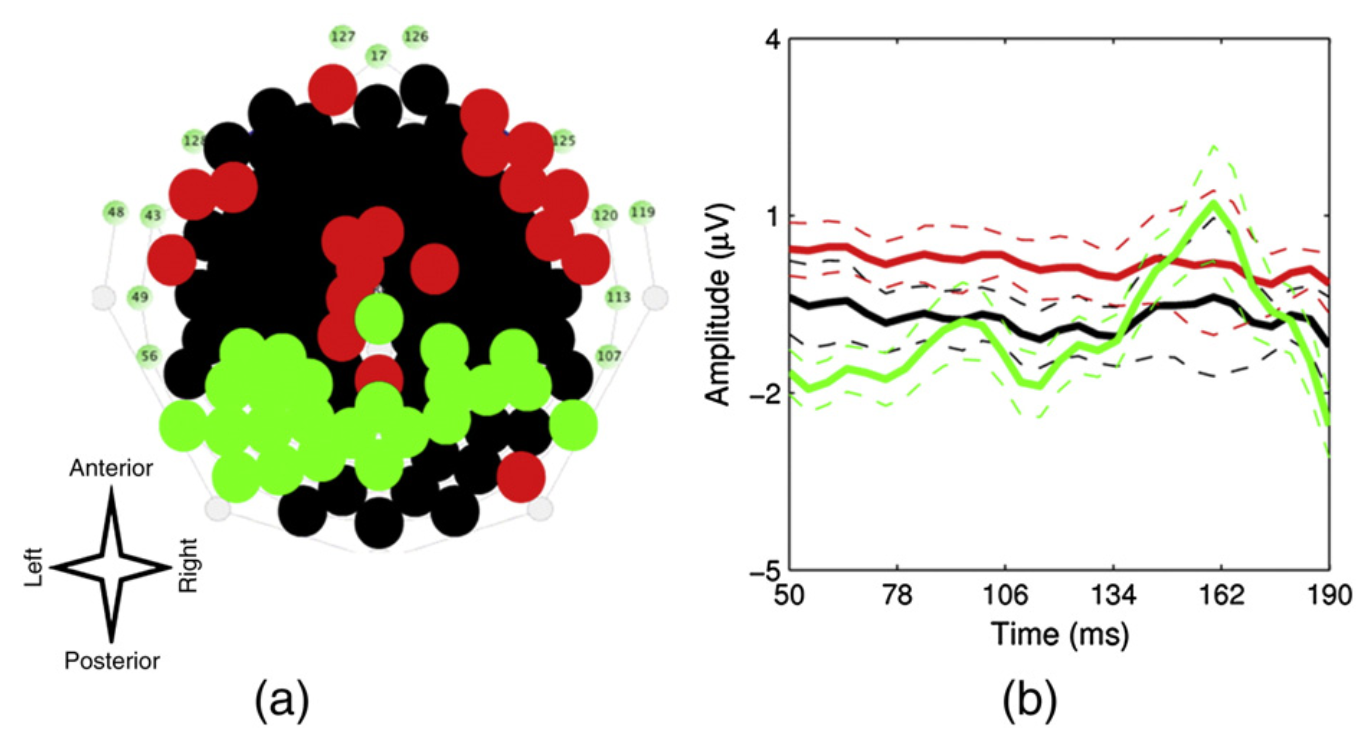
\includegraphics[width=0.75\linewidth,keepaspectratio]{eeg_erp_location}
\caption[Example of an ERP]{A 2D mapping of the electrodes and their group averaged waveform (solid lines). The standard deviations of the channel averaged are given as the dashed lines. Image sourced from Karamzadeh et al.\cite{Karamzadeh2013}.}
\label{fig:erpExample}
\end{figure}
%%%%%%%%%%%

\paragraph*{Brain State/Workload}
Analysis of involuntary conditions address the state of a person's brain which can refer to the emotional state, disease state, or attention/workload state. Those afflicted with Alzheimer's \cite{Jeong2004}, alcoholism \cite{Porjesz2005}, and mental disorders such as \ac{ADHD} and Bi-Polar disorder \cite{Basar2008} present with distinct \ac{EEG} features. Knowing these conditions can manifest in the \ac{EEG} recordings provides context for the how the known underlying biological changes alter a subject's \acp{EEG}. This is exemplified by studies measuring how stress impacts cognitive function \cite{Lupien2007} and a brain's workload during attention dependent tasks \cite{Schultze-Kraft2016}.

%%%%%%%%%%%%%%%%
\subsection{Algorithm Development}

The development of \ac{ML} techniques for \ac{EEG} tends to focus on areas well understood by clinicians, detecting seizures \cite{Chu2017,Wulsin2011}, identifying the stages of sleep \cite{Schluter2012,Hassan2016}, capturing \acp{ERP} \cite{Makeig2012,Guntekin2016}, or processing \ac{BCI} signals. Minimal focus has been given to a generalized classifier for interpreting multiple types of \acp{EEG} \cite{Vidaurre2011}. The approach closest to this goal is the use of \acp{EEG} for biometrics given that subject verification works on variety datasets with similar results \cite{Paranjape2001,Palaniappan2007a,Yang2016}. While conditional classification techniques (seizure detection, sleep classification, \acp{BCI}, and subject verification) are capable, they fail to increase our overall understanding of \acp{EEG}.

Despite the lack of a generalized classifier, the data specific classifiers rely on some amount of data pre-processing. This is necessary to address recording artifacts \cite{Lawhern2016,Mahajan2015,Minguillon2017}, optimize the available channel data \cite{Rocca2014}, or generate an acceptable feature set \cite{Su2018}.  In carrying out one or more of these pre-processing steps a preliminary amount of dimensionality reduction is introduced which becomes more pronounced as the data is windowed into epochs for a given algorithm \cite{Gross2014,Lotte2007b,Subasi2010}. 

Unfortunately all these steps are often unique to the type of \ac{EEG} being classified which means there is no well defined protocol of feature set that applies universally. For example, seizure algorithms typically process data in windows on the order of 10s of seconds \cite{Wang2016}. Biometric algorithms utilize channel subsets to verify a subject \cite{Campisi2014}. \acp{BCI} use spatial filters to target the regions of the motor cortex \cite{Schalk2004}. \acp{ERP} focus on the occipital region where recognition of stimulus is triggered \cite{Kindermans2014b}. Things are further complicated by the varying performance within a dataset based upon subject or recording variation seen in \ac{BCI} tasks \cite{Gross2014,Blankertz2007a,Kang2014b}, seizure recordings\cite{Ramgopal2014,Wulsin2011,Page2015}, and even biometric protocols \cite{Armstrong2015,Maiorana2016}. Due to this a comprehensive feature set remains elusive, but data specific feature sets have shown promise when paired with various algorithms.

These approaches leverage knowledge gained from the study of \acp{EEG} which makes them \emph{domain knowledge}. Unfortunately domain knowledge comes from clinicians which means, as outlined previously, there are limits to its impact. It is critical in understanding artifacts and background (Figure \ref{fig:wulsin_anno}), seizures (Figure \ref{fig:generalized_seizure}), and sleep patterns (Figure \ref{fig:sleep_spindle}) \cite{Bodizs2009,Wendt2012}, but clinicians have minimal knowledge specific to biometrics \cite{Paranjape2001}. Thus some approaches are bootstrapped by domain knowledge, but it furthers a Catch-22. Algorithms are made dependent clinician supplied insights when the algorithms task is to provide annotations to assist those same clinicians.

%%%%%%%
\begin{figure}
\centering
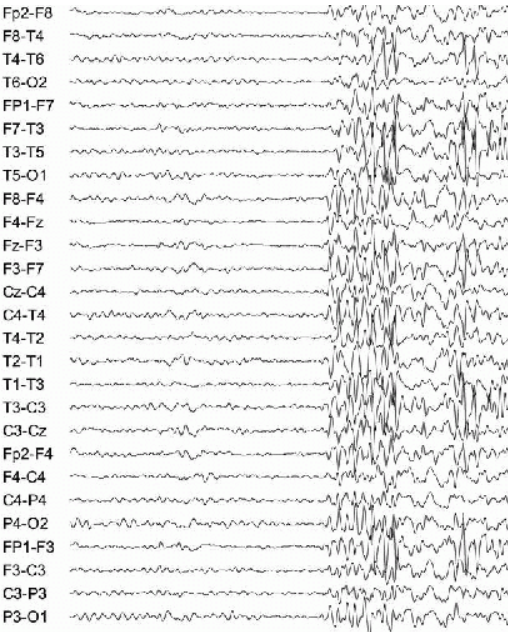
\includegraphics[width=0.6\linewidth,keepaspectratio]{generalizedSeizure_small}
\caption[Sleep Spindle example]{Sleep Spindle example drawn from the text of Tatum\cite{Tatum2014}. Notice the abrupt change in all recorded channels.}
\label{fig:generalized_seizure}
\end{figure}
%%%%%%%

%%%%%%%
\begin{figure}
\centering
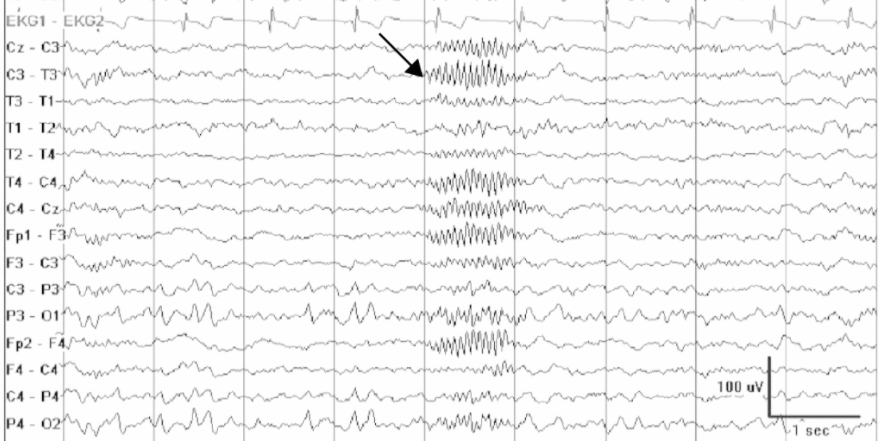
\includegraphics[width=0.6\linewidth,keepaspectratio]{sleepSpindles_small}
\caption[Sleep Spindle example]{Sleep Spindle example drawn from the text of Tatum\cite{Tatum2014}. The black arrow indicates the location of a sleep spindle which is captured across multiple, but not all, channels.}
\label{fig:sleep_spindle}
\end{figure}
%%%%%%

Within this loop of clinician annotations driving the development progress of algorithms, is the closed set of available \ac{EEG} datasets. Aside from the \ac{PNET} \cite{Goldberger2000} and \ac{BCI} competition \cite{Blankertz2006a} databases, much of the research is conducted on specific single use datasets \cite{Wulsin2011,Subasi2010,Radha2014}. Furthermore, when the \ac{PNET} database is used it is often the only dataset \cite{Yang2016,Marcel2007a,Fraschini2015,Rodrigues2016}. There are studies that combine datasets, but that they tend to focus on biometric applications \cite{Delpozo-Banos2015}.

This lack of a robust data landscape manifests as variable algorithm performance based on the dataset\cite{Lawhern2016,Lotte2007b} or, within the context of \ac{BCI} applications, as subjects being unable to use the system making them \textit{`illiterate'} \cite{Vidaurre2010a,Spezialetti2018}. This suggests there are intrinsic problems within processing \ac{EEG} data. Algorithm performance can they be viewed as being dependent on the type of data (\ac{BCI}, sleep, seizure, etc), but also the individual subjects themselves. This makes it difficult to tout any way forward given the lack of common performance benchmarks.

To address these data issues, algorithms must either be generalized, or built to tackle specific problems using domain knowledge. These two paths pair well with unsupervised (generalized) and supervised (specific) \ac{ML} algorithms \cite{Makeig2012,Martinez-del-Rincon2017,Blanco2010,Lotte2018}. The use of domain knowledge with supervised deep learning approaches have shown promise in \ac{BCI} \cite{Tabar2017}, sleep \cite{Aboalayon2014} and seizure \cite{Wulsin2011,Chu2017} classification. While their unsupervised counterparts do not require clinician support they do lag in comparative performance when addressing similar classification tasks \cite{Vidaurre2011,Lu2009a,Kasabov2013,Lotte2018}.

Efforts to address this data dependency in the \ac{BCI} field produced four styles of classification schemes: \emph{adaptive classifiers}, \emph{matrices and tensors}, \emph{transfer learning}, and \emph{deep learning}\cite{Lotte2007b}. Ten years on Lotte et al. \cite{Lotte2018} noted the same schemes work, but a focus should be placed on the end user. These reviews covered supervised and unsupervised algorithms indicating that no resolute classifier has been found for the \ac{BCI} community. Seizure classification has progressed, but the results are often using small esoteric datasets with 5 subjects \cite{Acharya2018} and 17 subjects \cite{Chu2017}. Biometric techniques continue to perform well, but have also failed to expand their datasets \cite{Abdullah2010,DelPozo-Banos2014a,Yang2016}.

The potential within the \ac{EEG} \ac{ML} community is vast. Presently performance varies based upon dataset, feature set, algorithm, and often subject quality. While some applications have become robust, seizure, \ac{ERP}, and \ac{BCI} classification show promise, this field is still maturing. Given the nascent status of \ac{EEG} processing borrowing techniques from an established domain may be helpful. In general much of the technology currently deployed for \ac{ML} pursuits comes from the realm of speech recognition, such as the time tested \ac{HMM} \cite{Rabiner1989}. Following this trend, the development of the unsupervised learning technique called \acp{IV} could offer growth of performance and understanding for \ac{EEG} classification tasks \cite{Kenny2008b}. \acp{IV} are able to learn decision surfaces for the accent, age, content, gender, and language of a speaker \cite{Behravan2016}. Through a series of data modeling utilizing \acp{GMM} \cite{Reynolds2009} that produce a \ac{UBM} \cite{Hasan2011} capturing the variability of the training data in a \ac{TVM}, it is possible to reduce the dimensionality of various sized segments of data into robust discrimination vectors, \acp{IV} \cite{Dehak2011a}.

%%%%%%%%%%%%%
\section{Research Proposal}

A clinician's primary focus is to treat their patients. Asking clinicians to produce perfectly annotated recordings to support algorithm research is not in the best interest of their patients or their overall productivity. There is little sense in asking clinicians for help to build datasets for algorithms who's goal is to reduce the time clinicians spend reading \acp{EEG}. This is clearly a Catch-22:  The people that algorithms can help must first help to train the algorithms. However, clinicians do not have the time or group consensus to meet the needs of the algorithms.

The most direct solution is to find a way to annotate recordings without involving clinicians. As discussed \ac{ML}-based solutions exist, but the field is diverse and lacks an apex technique. Despite the success of these techniques, fundamental problems continue to exist which must be overcome by all algorithms. These include variations in the quality of the recordings, the presence of adequate (in quality and quantity) annotated data, an acceptable feature set, and consistent channel layout across recordings. At its core the issue is identifying what characteristics of the \ac{EEG} are relevant for a given classification task. In most instances, annotated data and prior knowledge is leveraged in order to reduce the dimensionality, and thus the uncertainty, in the algorithm's classification. This approach reinforces a reliance on annotators, which is not ideal given the disparate quality and consensus of annotations.

Annotation-based techniques are presently the dominant \ac{ML} approach to classifying data. This means that clinicians effectively control the algorithms' performance which makes them an external source of error. To alleviate this constraint, unsupervised \ac{ML} algorithms can be developed to match the capabilities of their supervised counterparts. The benefits of equivalent performance would be significant, as unsupervised \ac{ML} enables training on large diverse datasets without the need of clinicians. Countless hours of data in need of annotation could thus be labeled, producing a steady supply of data for training supervised \ac{ML} algorithms and clinicians. By using \acp{IV} for this process it may also be possible to uncover novel phenomena in the data similar to their use on speech signals.

%%%%%%%%%%%%%%%
\subsection{The Research Aims}

The goal of this work was to lay the foundation for an unsupervised \ac{ML} system that classified and clusterd \ac{EEG} recordings. The preliminary pre-dissertation work indicated it was possible for \acp{IV} to perform subject verification and to sort data by similarity\footnote{See chapter 4's preliminary experiment results.}. While promising, these results had to be expanded to determine whether \acp{IV} could overcome the annotation advantage. This primarily relied on the constrained modeling processing carried out in the generation of \acp{IV}. Once mastered, the process was largely transparent in its approach making it possible to study the decision surfaces used for the proscribed classification and clustering tasks.

In addition to understanding how the proposed system operated on \acp{EEG}, it was necessary to prove that \acp{IV} could offer comparable performance to existing standard methods, including both \ac{ML} algorithms and clinicians. However, given the advancement of \ac{ML} algorithms, the ability to cluster and verify subjects is related only to algorithms. Clinicians do perform similar tasks, but they use resources beyond \ac{EEG} recordings to make their assessments such as medical reports. Thus the performance of \acp{IV} was evaluated against other well documented \ac{ML} of varying complexity to highlight the tradeoffs between performance, dimensionality reduction, and algorithm complexity.

From these areas of interest, three research questions were posed:

\paragraph*{Research Aim 1:} Can an \ac{IV}-based classification perform as well as, or better than, other applicable \ac{ML} techniques?
\paragraph*{Research Aim 2:} Under what conditions does an \ac{IV} based system perform best?
\paragraph*{Research Aim 3:} What characteristics of \ac{EEG} data do \acp{IV} take advantage of in their discrimination? Is this process inherently well suited for addressing \ac{EEG} classification?
\bigskip

By answering these questions, insight into the nature of \acp{IV} and \acp{EEG} was gained. This was possible because similar \acp{IV} work in the speech recognition community produced strong results related to subject verification \cite{Kenny2015}, language classification \cite{Li2013a}, accent detection \cite{Behravan2016}, and speaker age estimation \cite{Bahari2012}. The underlying hypothesis was that \acp{EEG} had a bounded mathematical space similar to speech signals. This space can be exploited by the constraints of the \ac{TVM} which shapes the \acp{IV} producing nuanced classification similar to those seen in speech.

%%%%%%%%%%%%%%%%%
%\subsection{The Research Motivation}

% This section is really nice and well written but its stuff you've already said before. This is basically restating the motivation laid out in the previous 20-odd pages. So what do I do?

%The reason to carry out this work is the clinical and academic need for annotated \ac{EEG} recordings. A Catch-22 exists in that the best supervised \ac{ML} techniques require a strong foundation of knowledge, consisting of labeled data, to produce results on par with trained clinicians. Without a peer-reviewed training dataset algorithms are unable to adequately annotate unlabeled datasets. The algorithms are beholden to the bias of the clinicians. Clinicians are biased by their training and experience, of which will never be comprehensive for all use cases of \acp{EEG}.

%This lack of universality means ground truth data must be produced for the training of supervised algorithms and clinicians. While clinicians would be the ideal source for this data, their time is better spent with their patients and they lack consistent inter-rater agreement. As supervised \ac{ML} approaches are reliant on annotated data, their performance suffers when they are trained on data that comes from unreliable sources. This suggests a third approach, unsupervised \ac{ML}, is needed to support the continued development of supervised \ac{ML} algorithms and clinicians.

%Unsupervised \ac{ML} is not without its drawbacks, largest among them a dependency on an equitable distribution of data. Fortunately the availability of \ac{EEG} is the easier to address than the availability of accurately annotated \ac{EEG} data. While there have always been numerous publicly accessible datasets, the existence of the \ac{TUHEEG} suggests there many be enough data available to adequately train an unsupervised algorithm. It is through these databases and advanced unsupervised \ac{ML} techniques it is possible to deepen our understanding of \acp{EEG} because the approach is mathematical and free from external sources of bias.

%Part of expanding our \ac{EEG} knowledge centers on formalizing how the data should be processed. A substantial amount of research focuses on finding the best feature-algorithm combination for given classification tasks. This is due to the disparate nature of the conditions, subjects, and study protocols. \acp{IV} are built on \acp{UBM} and \acp{TVM} that strive to constrain the relationships between the natural modes of the data while providing dimensionality reduction. This makes \acp{IV} an enticing option at encapsulating the disparity between datasets while producing transparent decision surfaces.

%From these decision surfaces it should be possible to expand our knowledge of \acp{EEG} through the statistically modeling that produces \acp{IV}. The ability to simultaneously classify and cluster datasets provides the ability to explore the impact of variations in features and training data. Accepting the imperfect nature of unsupervised \ac{ML} means that imperfect results are accepted and encouraged. These edge cases should provide insight into the functionality of \acp{IV} as they are deployed onto a new type of data. From these insights relationships between \ac{EEG} data and features should all be possible helping close the loop on \acp{EEG} annotations.

%%%%%%%%%%%%%%%%%%
\subsection{The Research Experiments}

The Aims of this work was addressed in three experiments: \emph{Parameter Sweeps}, \emph{Algorithm Benchmarks}, and \emph{\ac{UBM}-\ac{TVM} Relationship}. Upon completing the experiments, the process of producing \acp{IV} from \ac{EEG} data was understood along with which properties of \ac{EEG} and \ac{IV} made this approach viable for producing annotations in an unsupervised manner.

\paragraph*{Parameter Sweeps}
The purpose of the \emph{Parameter Sweeps} was to determine optimal operating parameters for applying \acp{IV} to \acp{EEG}. This addressed Research Aim 2 by measuring the significance of specific features, channels, \ac{UBM} mixture sizes, and the \ac{TVM} training process. Testing each parameter over a range of values produced trends for a best practice approach to baseline \ac{IV} systems. The statistical decomposition of each dataset (abnormal, normal, motion trials, and seizure) and \ac{IV} development process provided background and baseline results enabling comparisons against the other published results where the data is not publicly available.

\paragraph*{Algorithm Benchmarks}
In order to validate \acp{IV} as an option for classification and clustering of \ac{EEG} data their performance was compared against a suite of \ac{ML} algorithms. The algorithms were evaluated through their sensitivity and specificity and, when applicable, their ability to cluster. These experiments addressed Research Aim 1 through a series of \ac{LOOCV} experiments based on subject and channel classifications.  

\paragraph*{\ac{UBM}-\ac{TVM} Relationship}
The relationships between \acp{UBM} and \acp{TVM} was deconstructed to examine the trade-offs made during optimization of the \ac{TVM}. Using the reported performance of \ac{GMMUBM} and \ac{IV} classifications, the influence of the mixture weighting were traced throughout the entire modeling process. This manifested as comparative feature and mixture mappings for each classification test. These mappings unlocked the fundamental statistical properties used to differentiate subjects which can then be compared across data sets as they are bounded by a common feature set. Ultimately this protocol turned \acp{IV} into a powerful multi-modal signal analysis technique.